\begin{frame}{Scrabble Result: Evolvability Signature}

\begin{figure}
  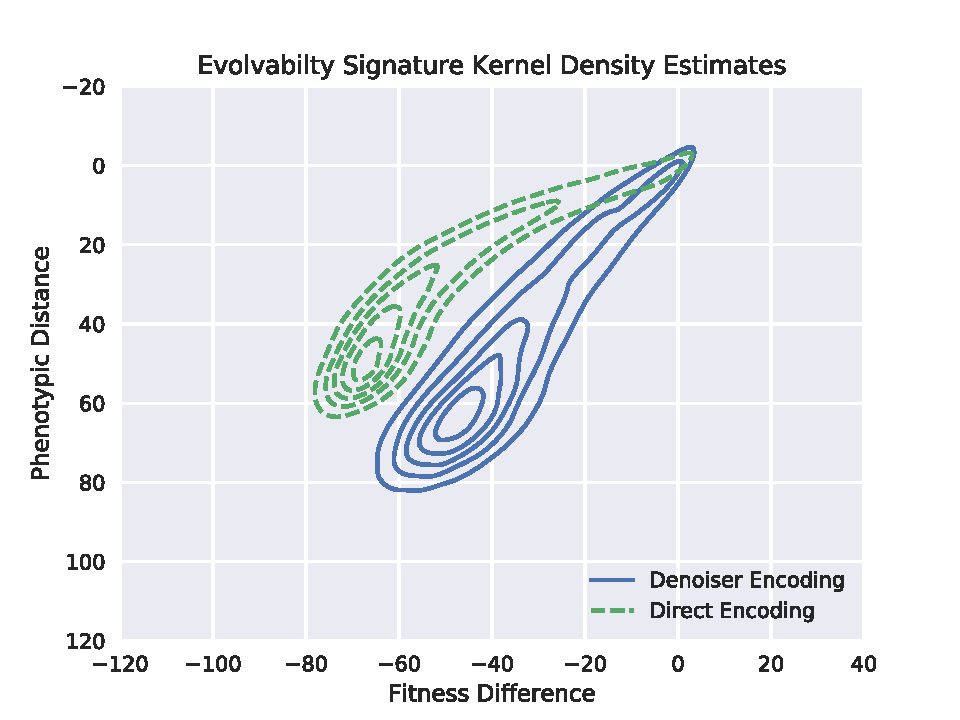
\includegraphics[width=0.8\linewidth]{img/results/scrabble_es_kde}
  \caption{
    Gaussian kernel density estimates for evolvability signatures of direct and indirect encodings in Scrabble string domain \cite{tarapore2015evolvability}.
  }\label{fig:scrabble_es_kde}
\end{figure}


\end{frame}

\begin{frame}{Toy Result: Evolvability Signature}

\begin{figure}
  \begin{subfigure}[b]{0.33\linewidth}
    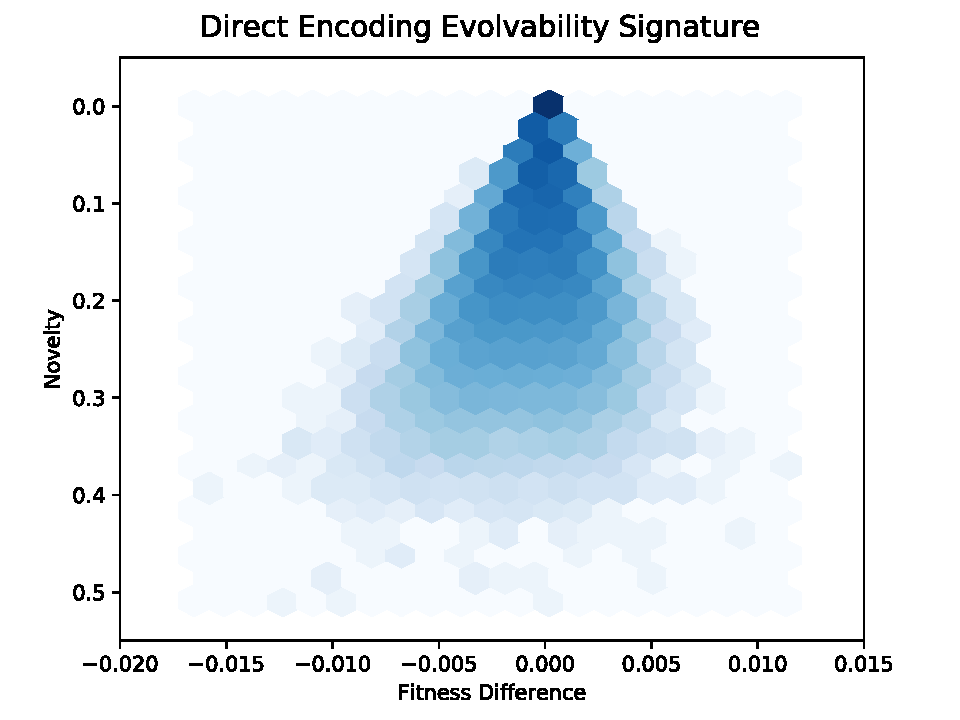
\includegraphics[width=\linewidth]{img/results/direct_es_unscaled}
    \subcaption{
      direct map
    }\label{fig:table_direct_es}
  \end{subfigure}
  \begin{subfigure}[b]{0.33\linewidth}
    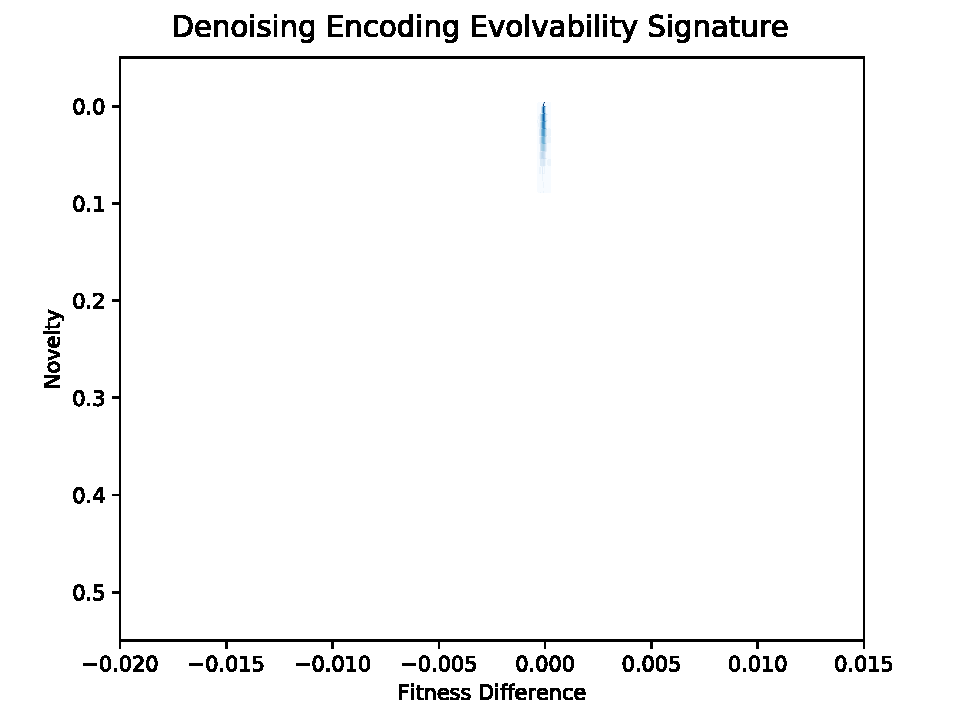
\includegraphics[width=\linewidth]{img/results/noise_es_unscaled}
    \subcaption{
      denoising map
    }\label{fig:table_noise_es}
  \end{subfigure}
  \begin{subfigure}[b]{0.33\linewidth}
    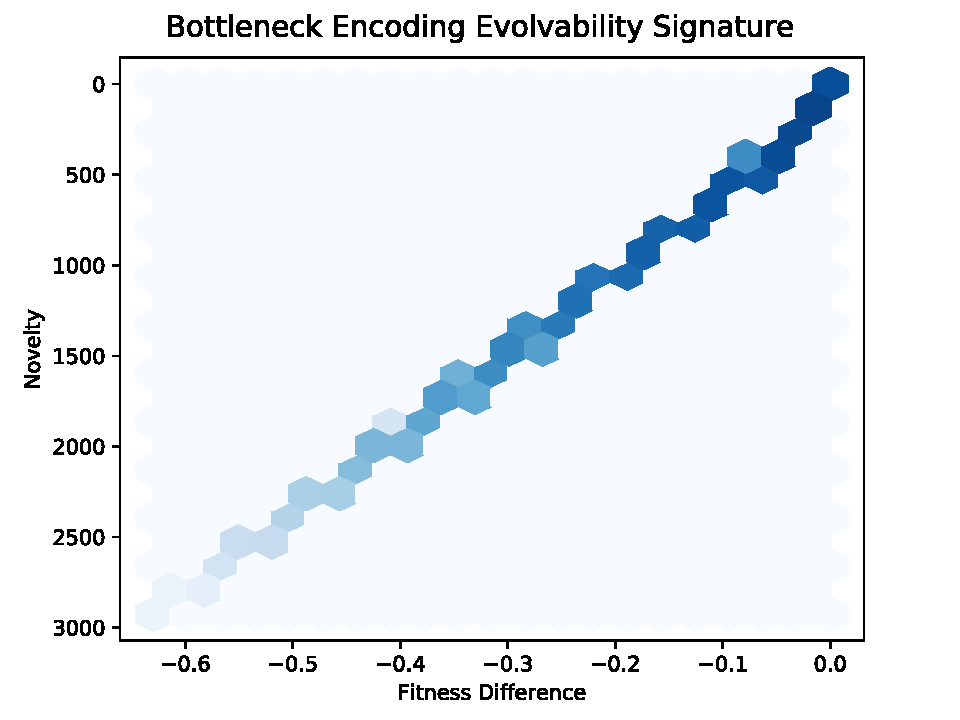
\includegraphics[width=\linewidth]{img/results/bottleneck_es_unscaled}
    \subcaption{
      bottleneck map
    }\label{fig:table_bottleneck_es}
  \end{subfigure}
  \caption{
    Evolvability signatures for three genotype-phenotype maps in the $n$-legged table problem domain.
    Note that subfigure \ref{fig:table_bottleneck_es} is presented with different axis scaling than subfigures \ref{fig:table_direct_es} and \ref{fig:table_noise_es}.
  }\label{fig:all_es}
\end{figure}


\end{frame}

\begin{frame}{TODO}

\begin{figure}
\foreach \n in {6,...,1}{%
\includegraphics[width=0.167\textwidth]{curly-guy/linear-\n}%
}%
\caption{TODO}
\end{figure}

\end{frame}

\begin{frame}{Result: Evolutionary Pacing}

\begin{figure}
  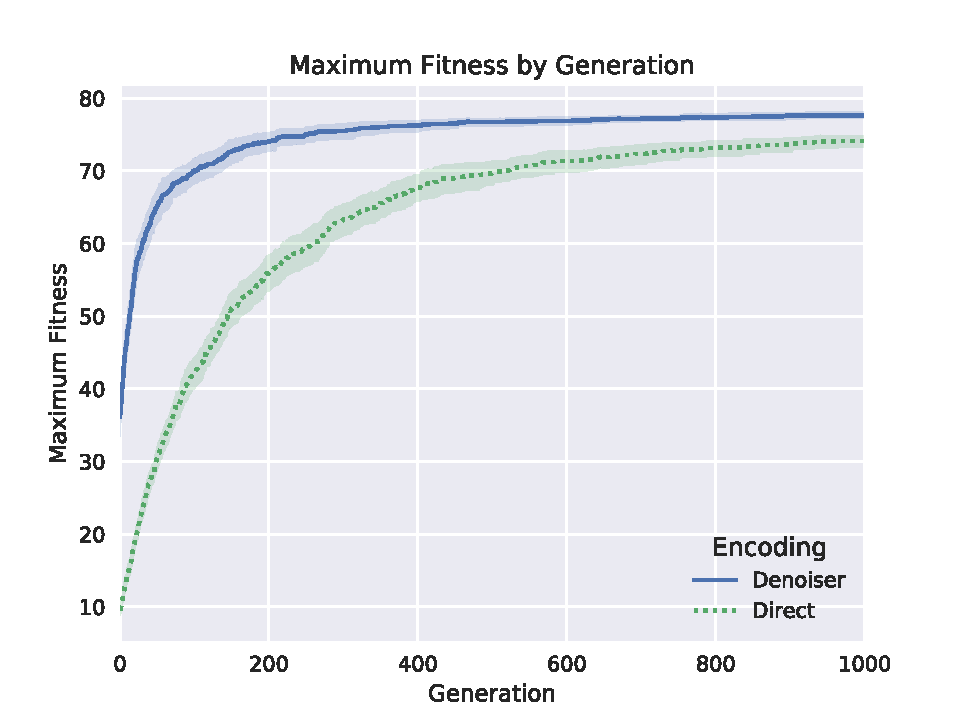
\includegraphics[width=0.8\linewidth]{img/results/scrabble_fit_vs_gen}
  \caption{
    Maximum individual fitness by generation in populations evolving in the Scrabble string domain.
    Bootstrapped 95\% confidence intervals are shaded along each curve.
  }\label{fig:scrabble_fit_vs_gen}
\end{figure}


\end{frame}


% \begin{frame}{Evolutionary Algorithm Parameters: Toy Problem}
%
% \begin{itemize}
% \item population size: 300
% \item tournament selection: $k = 5$
% \item crossover: two-point, two-parent, $p = 0.5$
% \item mutation: site-wise Gaussian perturbation
% \begin{itemize}
% \item training data, evolvability-signature experiments: $\mu = 0$, $\sigma = 0.1$, per-individual
% probability = 0.2, per-site probability = 0.01
% \item response-to-selection experiments: $\mu = 0$, $\sigma = 0.1$, per-individual probability = 0.2, per-site probability = 0.2 %TODO check this
% \footnote{for the bottleneck map, a per-site probability of 1 was employed}
% \end{itemize}
% \end{itemize}
%
% \end{frame}
%
% \begin{frame}{Denoising Autoencoder Hyperparameters: Toy Problem}
%
% \begin{itemize}
% \item 100-to-100 fully-connected linear layer without bias
% \item trained for 2500 epochs by stochastic gradient descent
% \item learning rate: $10^{−4}$
% \item momentum: 0.9
% \item batch size: 2048
% \item model parameters initialized uniformly between 0.005 and 0.015
% \item model parameters clamped in the range (0, 1
% \item during the training process, Gaussian
%   noise with $\mu = 0$, $\sigma = 0.025$ applied to input
% \item loss: mean square error of the difference between the original phenotype the reconstructed phenotype
% \end{itemize}
%
% \end{frame}
%
% \begin{frame}{Evolutionary Algorithm Parameters: Scrabble Problem}
%
% TODO
%
% \end{frame}
%
% \begin{frame}{Autoencoder Intuition: Bottlenecked}
%
% \begin{figure}
%   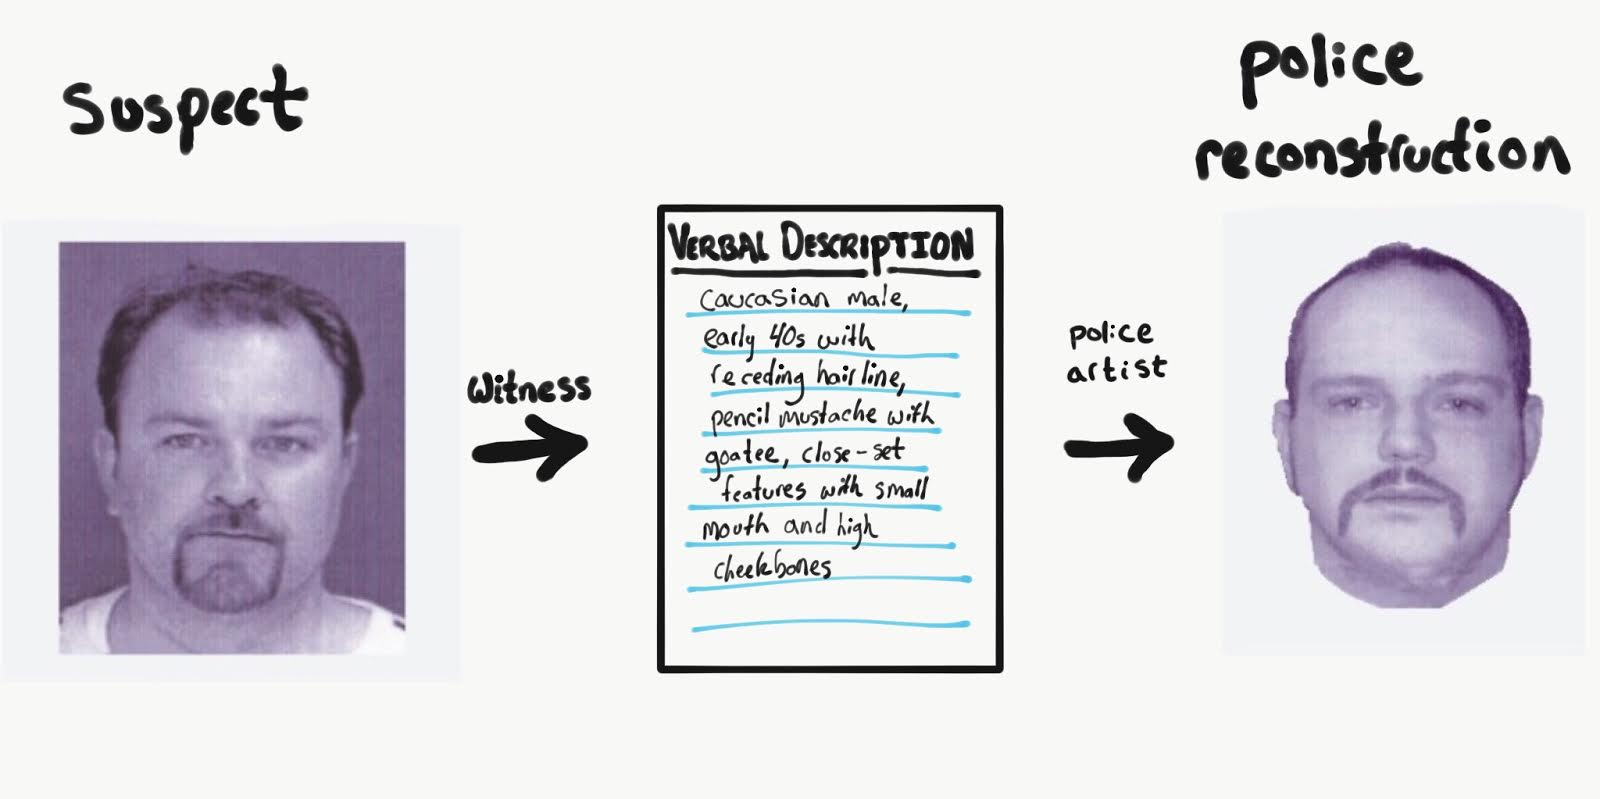
\includegraphics[width=\textwidth]{img/suspect}
%   \caption{
%   Schematic of hypothetical police composite process. Mug shot and composite reconstruction were taken from the Crime Scene Training Blog.
%   TODO cite
%   }
% \end{figure}
%
% \end{frame}
%
% \begin{frame}{Autoencoder Intuition: Denoiser}
%
% \begin{figure}
%   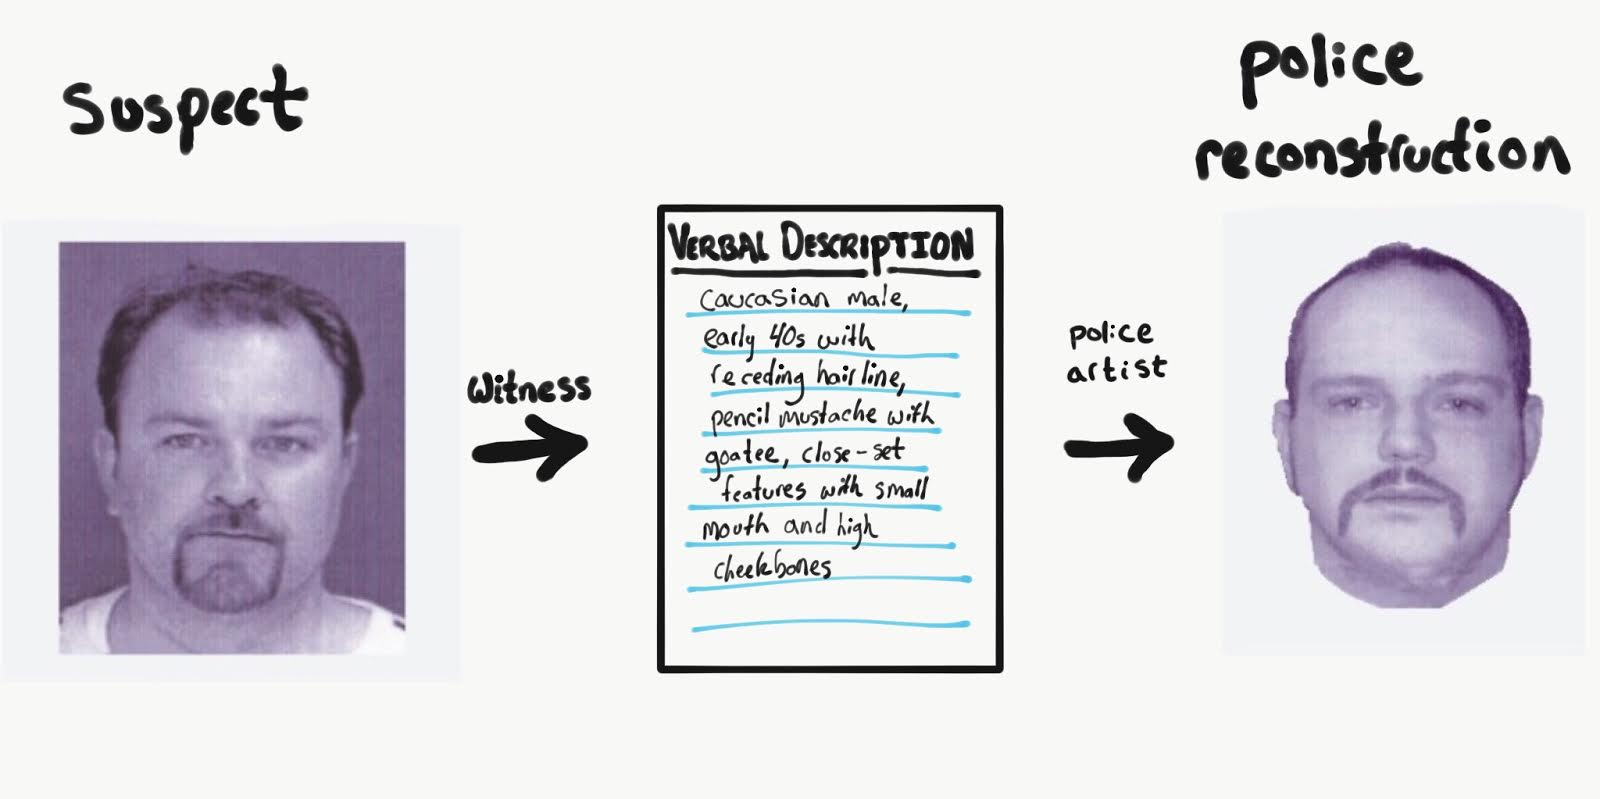
\includegraphics[width=\textwidth]{img/suspect}
%   \caption{
%   Schematic of hypothetical police composite process with suspect in disguise (incomplete input). Mug shot and composite reconstruction were taken from the Crime Scene Training Blog.
%   TODO cite
%   }
% \end{figure}
%
% \end{frame}
